%!TEX root = ../dokumentation.tex
\section{ERMs}
\subsection{allink.planer}
Als Ausgangslage dient mir das ERM des allink.planer. Die Entitäten Person und Project werden mit dem Wochenplaner verknüpft.

\begin{figure}[!ht]
\begin{center}
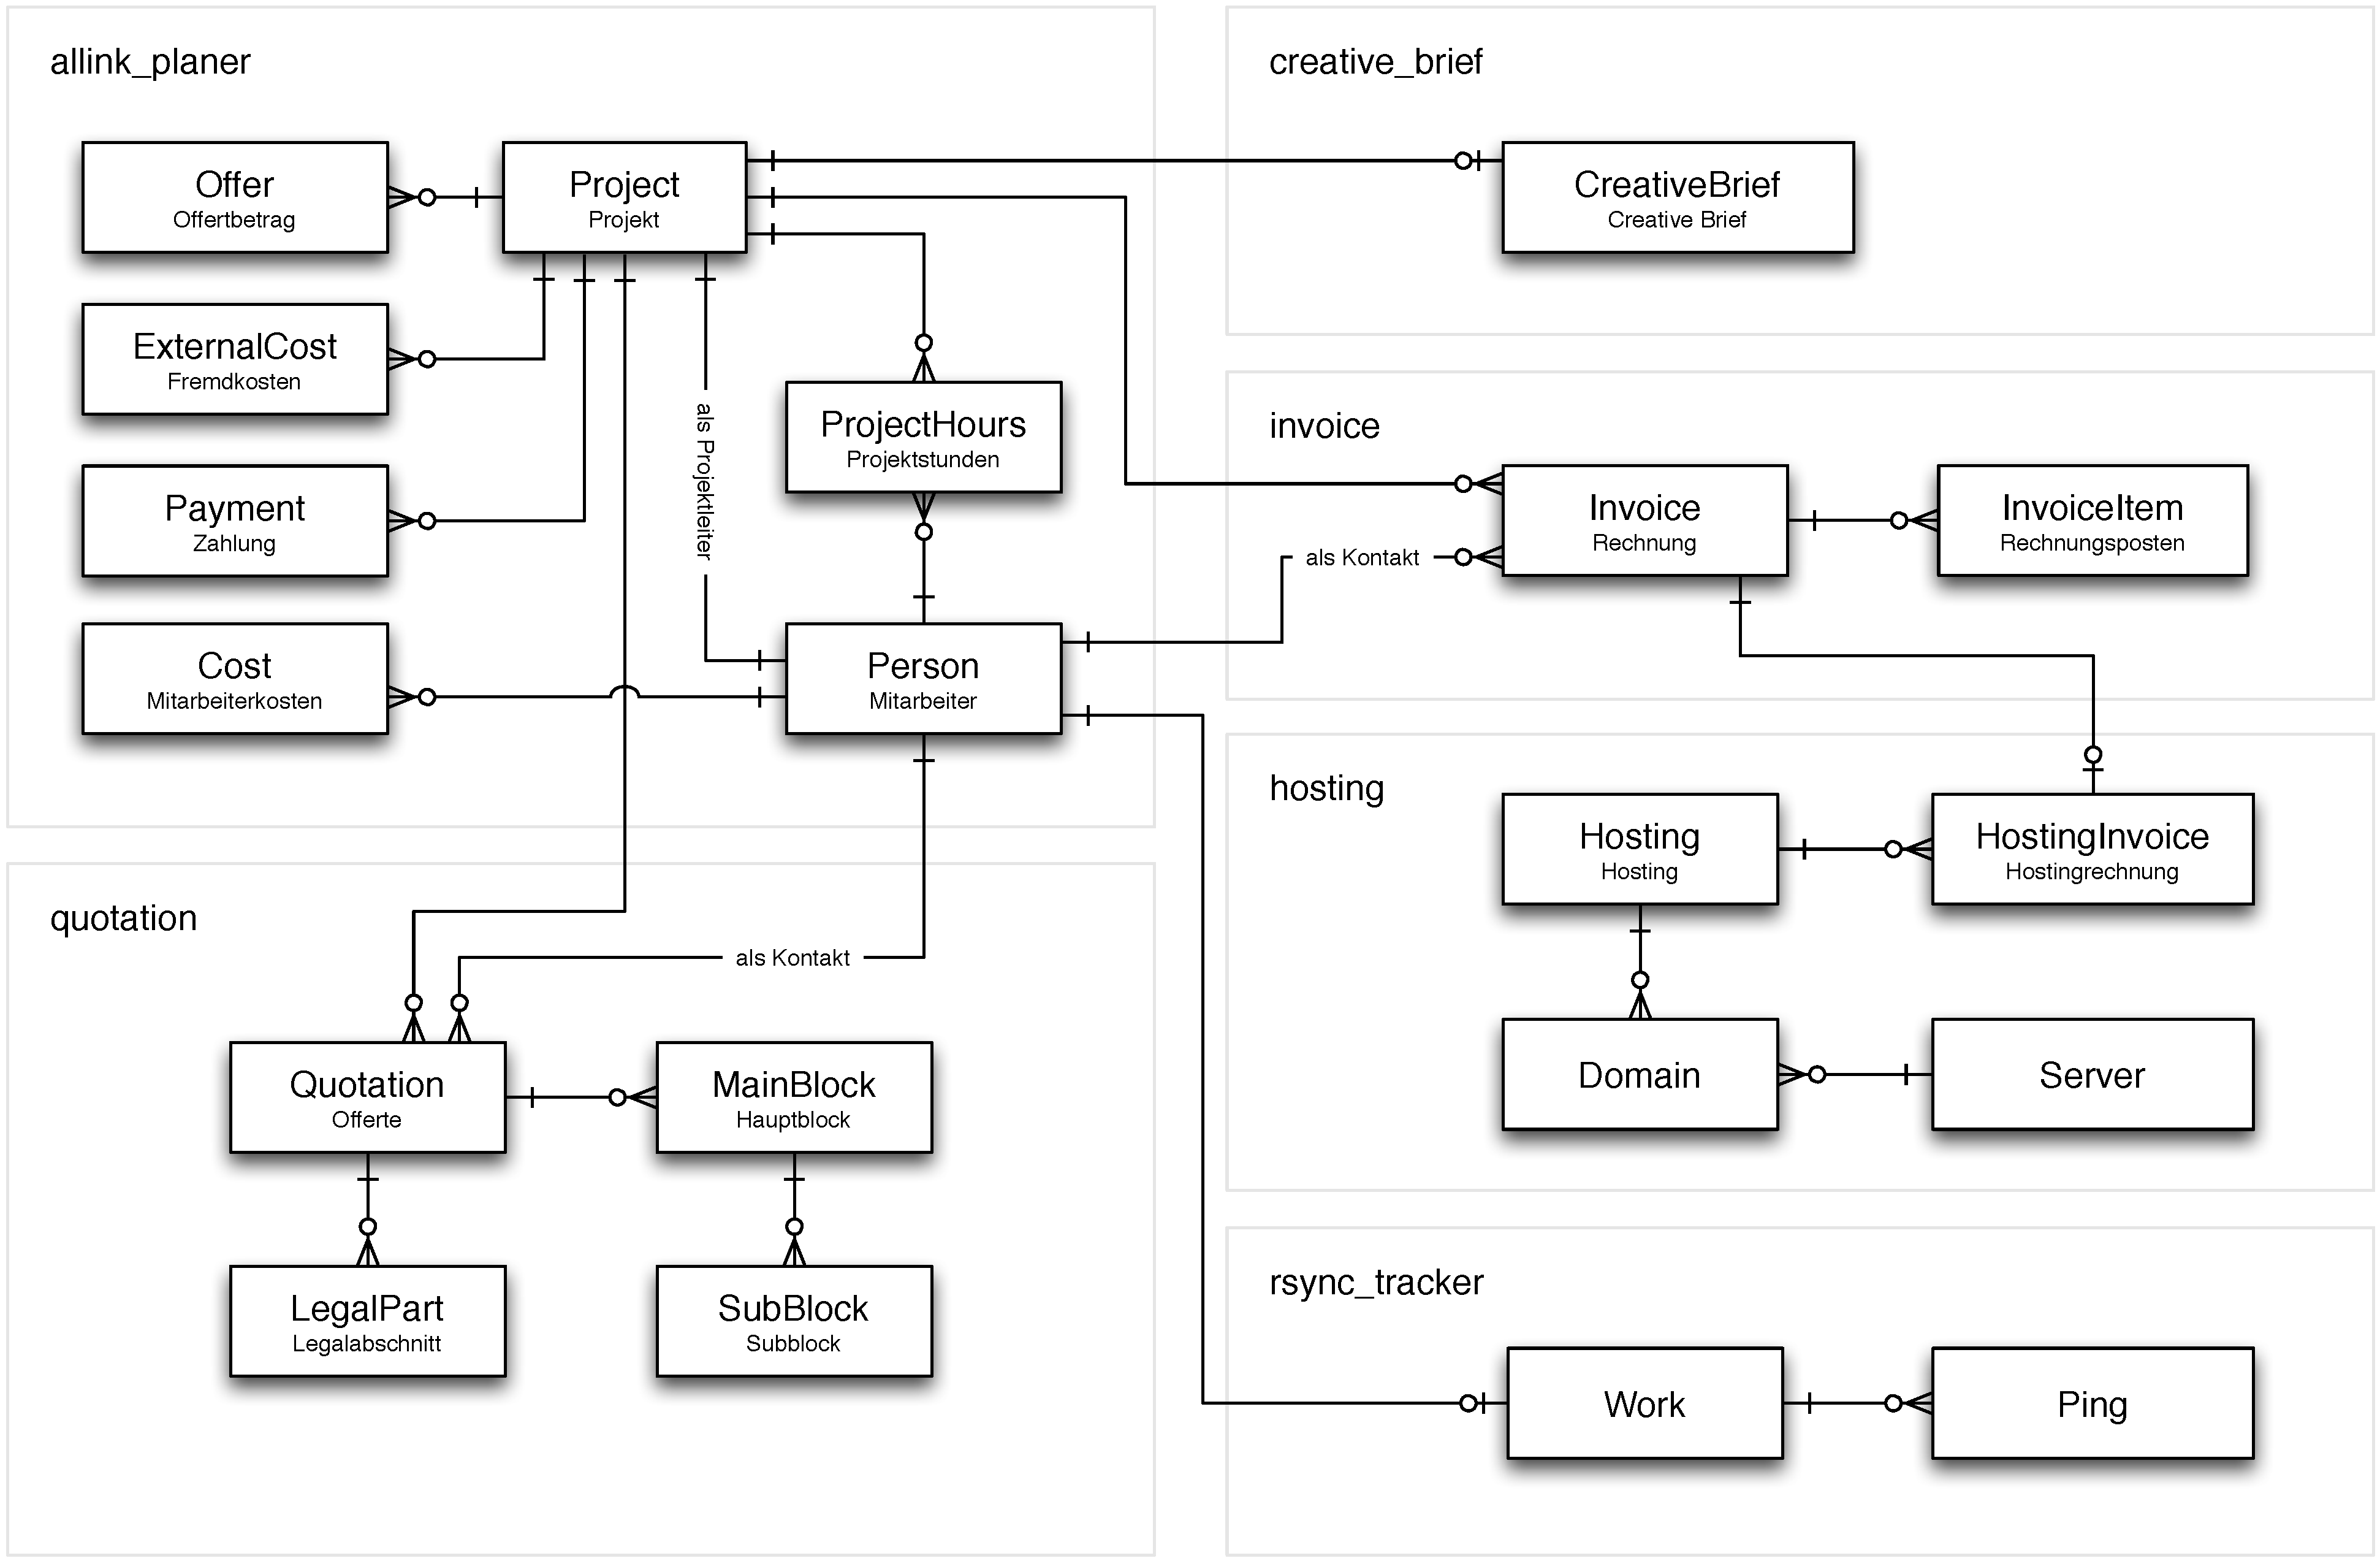
\includegraphics[width=0.99\textwidth,angle=0]{./bilder/erm_planer.pdf}
\caption[ERM allink.planer]{ERM allink.planer\footnotemark}
\end{center}
\end{figure}
\footnotetext{Entommen aus allink.planer}

\clearpage

\subsection{Wochenplaner}
\begin{figure}[!ht]
\begin{center}
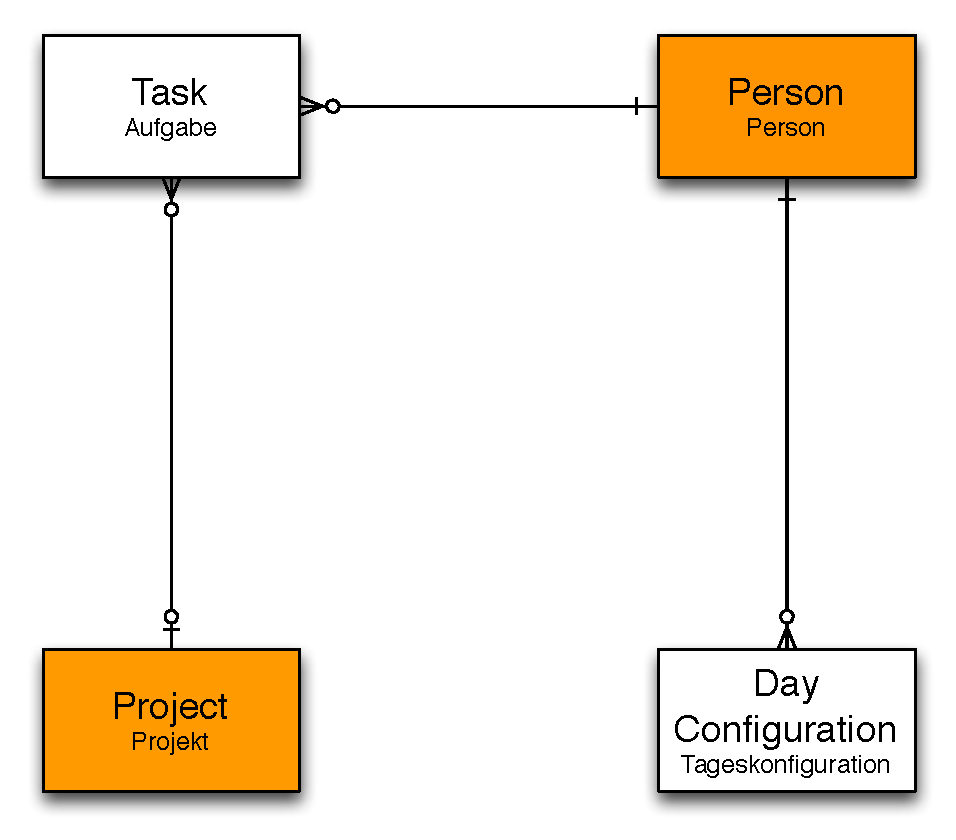
\includegraphics[width=0.5\textwidth,angle=0]{./bilder/erm.pdf}
\caption[ERM Wochenplaner]{ERM Wochenplaner (die Orange hinterlegten Entitäten stammen aus dem allink.planer)\footnotemark}
\end{center}
\end{figure}
\footnotetext{Eigene Darstellung}
\clearpage
\section{Design}
\subsection{Altes Design}
So sieht der momentane Wochenplaner aus:
\begin{figure}[!ht]
\begin{center}
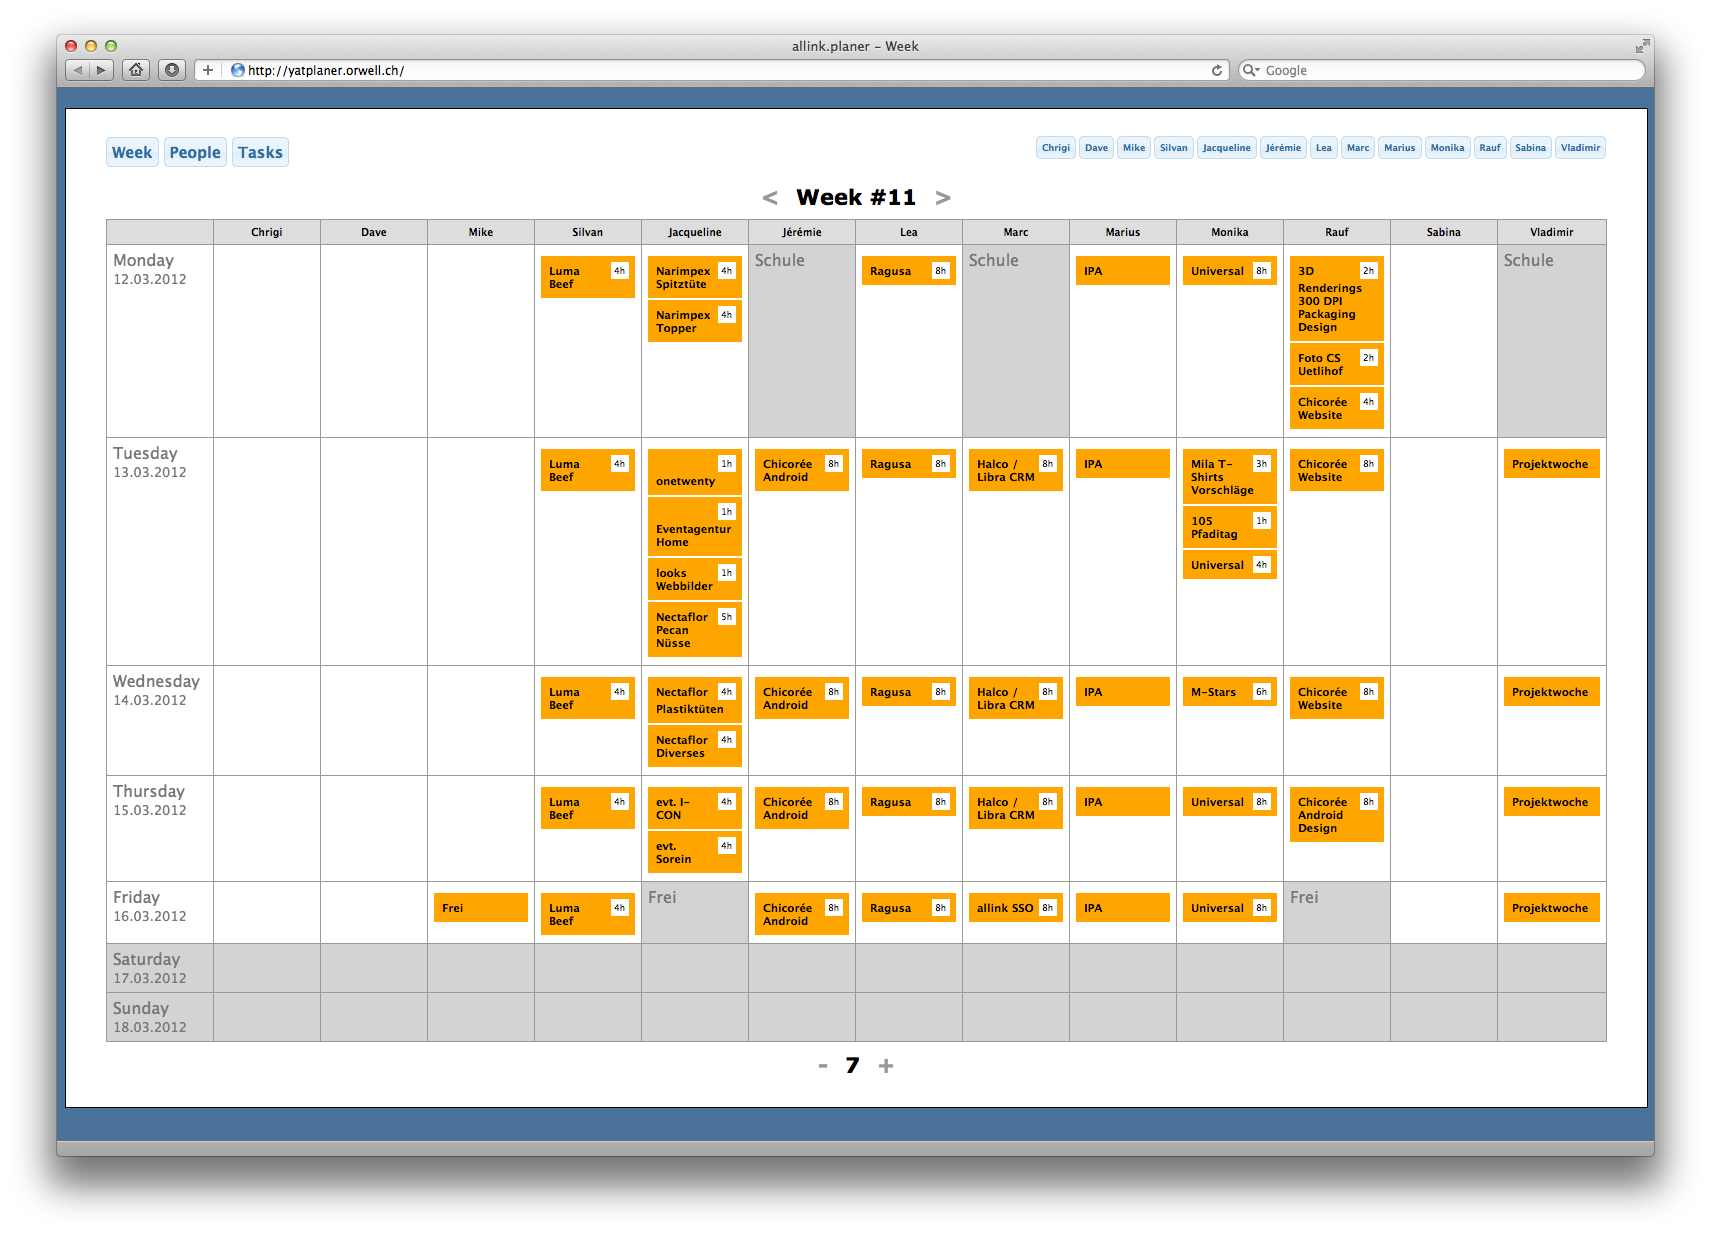
\includegraphics[width=0.99\textwidth,angle=0]{./bilder/yatplaner.png}
\caption{Bisheriges Design des yatplaner}
\end{center}
\end{figure}

\clearpage
\subsection{Neues Design}
Mit folgendem Design soll der Wochenplaner umgesetzt und an das allink CI/CO angepasst werden:
\begin{figure}[!ht]
\begin{center}
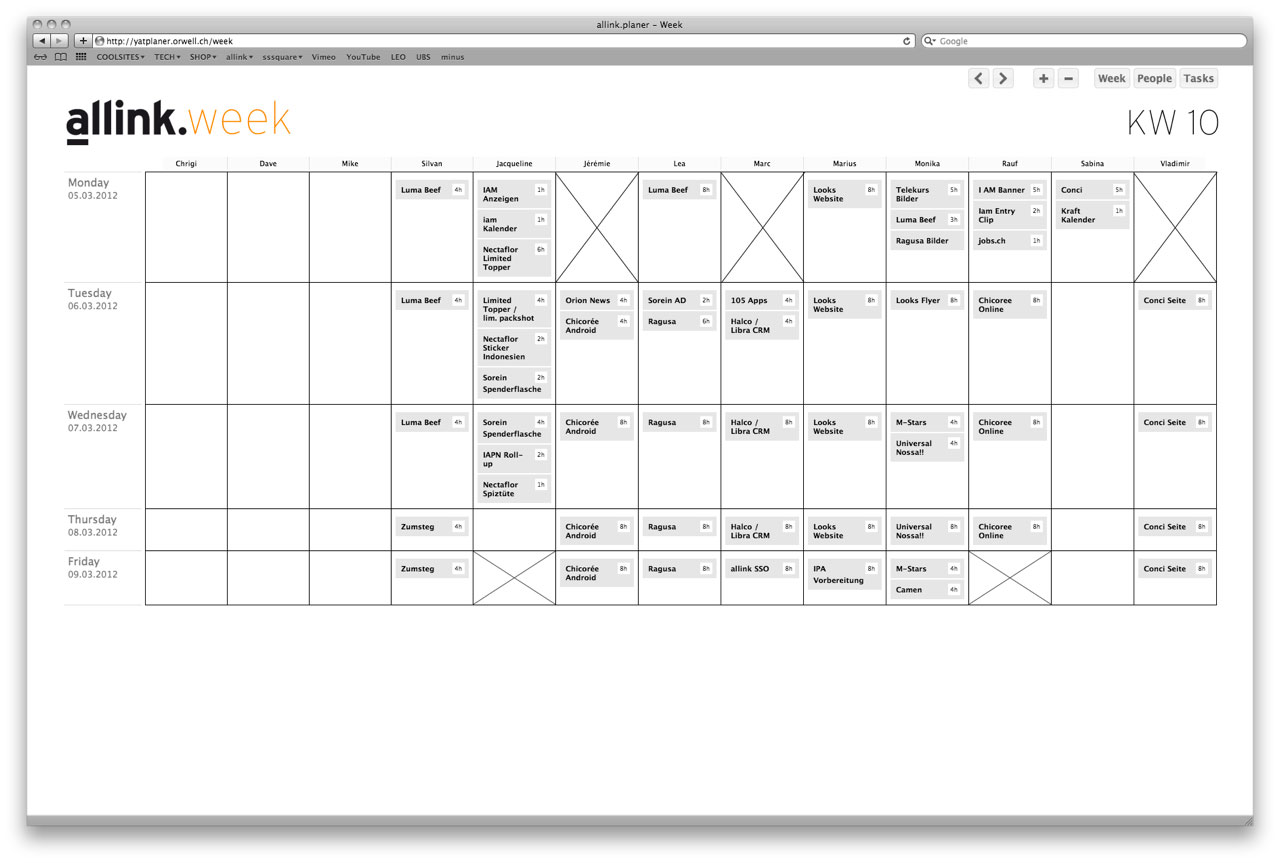
\includegraphics[width=0.99\textwidth,angle=0]{./bilder/wochenplaner.jpg}
\caption{Neues Design}
\end{center}
\end{figure}

%\section{System-Beschreibung}
\section{Umsetzung}
Da ich nicht auf die gesamte Entstehung des Quellcodes eingehen kann und der Verlauf im git-repository einsehbar ist,
führe ich die Umsetzung der Ziele auf.\\\\
Der Wochenplaner besteht aus 2 Bereichen in denen Daten manipuliert werden können:
\begin{itemize}
    \item Administrationsbereich (ist ein Standardfeature von Django um Applikationen zu verwalten)
    \item Wochenansicht (zusätzliche View im bestehenden Adminbereich)\\
\end{itemize}
Obwohl eine Intuitive Bedienung gefordert ist, müssen nicht alle Ziele in der Wochenansicht manipulierbar sein.\\
Die folgende Aufstellung zeigt auf welche Ziele wo umgesetzt wurden.\\

\begin{table}[!ht]
\begin{center}
    \begin{longtable}{llp{3cm}l}
        \toprule Ziel-Nr & Admin & Wochenansicht \\
        \midrule 1 & x & x \\
        \midrule 2 & x & x \\
        \midrule 3 & x & x \\
        \midrule 4 & x & x \\
        \midrule 5 & x & x \\
        \midrule 6 & x & x \\ 
        \midrule 7 & x &  \\
        \midrule 8 & x &  \\
        \midrule 9 & x &  \\
        \midrule 10 & x &  \\
        \midrule 11 & x &  \\
        \midrule 12 & x & x \\
        \midrule 13 & x & x \\
        \midrule 14 & x &  \\
        \midrule 15 & x &  \\
        \midrule 16 &  & x \\
        \midrule 17 &  & x \\
        \midrule 18 &  & x \\
        \midrule 19 &  & x \\
        \bottomrule
        \end{longtable}
    \caption{Funktionsbereiche der Ziele}
    \label{tab:funktionsbereiche_ziele}
\end{center}
\end{table}
\section{Resultat}
Das Resultat meiner IPA ist eine Webapplikation, in der Tasks über eine HTML-Ansicht per Ajax intuitiv verwaltet werden können. Die Applikation ist in das Projektmanagementtool allink.planer integriert.
Die Tasks sind mit Personen und Projekten verknüpft. Dadurch können in Zukunft diverse Analysen gemacht werden.
\section{Modellierung}
Über das Django-Framework kann man die Modelle der Klassen bzw. Entitäten erfassen.
Alle Modelle können als Applikationen über einen Administratorbereich durch CRUD manipuliert werden.
\subsection{Task}
\begin{itemize}
    \item Name (Char)
    \item Duedate (Date)
    \item Person (Fremdschlüssel)
    \item Duration (Stundenanzahl)
    \item Project (Fremdschlüssel)
    \item sortindex (int)
\end{itemize}
\subsection{Tageskonfiguration}
    \begin{itemize}
        \item Description (Char)
        \item Day (Int, ChoiceField)
        \item Person (Fremdschlüssel)
        \item startdate (Date)
        \item enddate (Date)
    \end{itemize}
\section{Layout}
Das Layout bleibt, bis auf einige kleine Anpassungen und das neue Design, dasselbe.\\
Im neuen Layout hat die Woche nur noch 5 anstatt 7 Tage und die Links zum admin-Bereich wurden versetzt.
% \section{Effektive Umsetzung der Applikation}
% Modelle erzeugt\\
% urls für wochenplaner
% Adminbereich eingerichte, App lebt im admin und muss von dort aus gesteuert werden\\
% \section{Templating Wochenansicht/Frontend}
% Template für Wochenansicht erstellt
% Daten werden an template übergeben
% Tage werden korrekt ausgeben
% Tasks sind an der richtigen Stelle (Tag und Person)
\section{Entwicklungsumgebung}
Die Entwicklungsumgebung besteht aus den in den Firmenstandards genannten Technologien.
% Als Betriebsystem verwende ich MacOS X, was (bis auf TextMate) aber nicht voraussetzend ist für das entwickeln mit Django.\\
% Django ist ein Python-Framework das sich auf eine schnelle Webentwicklung konzentriert (Details auf djangoproject.com).\\
% Über das Terminal verwalte ich eine virtuelle Python- und Django-Umgebung und das Versionierungssystem Git.\\
% Als Texteditor verwende ich TextMate. Ein schlichter aber funktionaler Editor der viele Bundles für Programmiersprachen anbietet.\\
% \section{Versionierungssystem}
% Als Firmenstandard wird Git bzw. Github verwendet. In den letzten Jahren ist Git in der Programmierszene sehr beliebt geworden und
% löst Subversion als Leader ab.\\
% Über Github können Repositories verwaltet werden und vereinfacht die Zusammenarbeit von Entwickler am selben Projekt sehr stark.
\section{Herausforderungen \& Entscheidungen}
\subsection{JSON}
Um dynamisch die Datenbank zu manipulieren, kann eine Methode in Django verwendet werden, über die Requests im JSON-Format an den Server geschickt werden. 
Über den django-piston Handler können diese Requests entgegengenommen und weitergeleitet werden.\\
Bis jetzt habe ich lediglich über einen JSON-Handler Daten aus der Datenbank gelesen oder neue Datensätze erstellt.\\
Einen bestehenden Datensatz zu ändern und diesen dann korrekt im Frontend wieder einzusetzen, ist ein bisschen knifflig, aber im Nachhinein doch sehr logisch zu verstehen.
Durch eine Einführung von Silvan Spross konnte ich diesen Prozess verstehen und nachvollziehen.
\subsection{Queries für Wochenansicht}
Bisher habe ich alle Objekte die ich in der Wochenansicht benötigt der View übergeben.
Im Template habe ich über die Objekte iteriert und die entsprechenden Daten ausgegeben. Dies ist jedoch nicht `schön'. 
Darum habe ich mit Unterstützung von Marc Egli, der mir die Verschachtelung von Tuples zeigte, die Objekte mit den korrekten Queries verschachtelt übergeben und dann im Template aufgelöst.
\subsection{JS Funktionalität (CRUD mit jQueryUI \& AJAX) }
Die Wochenansicht der Tasks ist eine rein statische Ansicht.
Alle Tasks und Sperrtage können über den Django admin per CRUD manipuliert werden. Dies ist aber nur ein Teil der bestehenden Funktionalität.
Es wird eine CRUD-Funktionalität im Frontend benötigt. Diese werde ich mit jQueryUI realisieren da ich mit jQuery am meisten Erfahrung habe und Firmenstandard ist.
Sich in Alternativen einzuarbeiten benötigt zu viel Zeit und ist nicht mit jQuery kompatibel.
Per jQueryUI können alle Tasks frei zu jedem Tag und/oder Person verschoben werden.
Per AJAX werden neue Tasks automatisch in die DB geschrieben und danach ins HTML eingefügt.
\subsection{Sperrtage}
Zuerst habe ich Sperrtage nur mit einem Tag versehen und später noch mit einem Startdatum.
Wenn man aber nachvollziehen will wer wie lange wann gefehlt hat, darf man einen Sperrtag nicht einfach überschreiben.
Also sind die Sperrtage auch mit einem Enddatum versehen. In der Abfrage für die Wochenansicht wird für jeden Tag geprüft,
ob ein Sperrtag beginnt, endet oder kein Enddatum angegeben ist.
Somit müssen keine Sperrtage gelöscht werden und es sind mehrere erfassbar, die sich automatisch ergänzen.
\subsection{Task duplizieren per jQueryUI}
Wie man einen Task per AJAX dupliziert ist auf verschiedenen Weisen möglich.\\
Zuerst habe ich es über ein sogenanntes Cloning versucht in dem eine Kopie des Tasks erstellt wird und dann als neuer Task eingesetzt werden kann.
Da ich wusste, dass dieses Feature umfangreich wird, habe ich es in einen separaten ``branch'' ausgelagert.
Jedoch stiess ich dabei auf grosse Probleme in der Umsetzung, da das cloning zusätzlich mit einer gedrückten Tastenkombination erfolgen sollte.
Nach einer Besprechung mit der Projektleitung wurde beschlossen, dass den Task über einen Button dupliziert und unten eingesetzt wird.
\section{Semantische Codebehebungen}
Am Ende des Testings habe ich zur Erhöhung der Codequalität eine Codesäuberung mit pep8, pyflakes und jshint vorgenommen. Dabei wird falsche Syntax und
nicht verwendete Imports hervorgehoben.
% \section{Implementierung}
% Der Wochenplaner kann als App mit Abhängigkeiten (Person, Projekt, piston, jQueryUI) in den allink.planer direkt integriert werden.
